\documentclass[a4paper,10pt]{article}

\usepackage[utf8x]{inputenc}
\usepackage{microtype}
\usepackage[DIV=20]{typearea}

% \usepackage{geometry}
% \geometry{
% 	margin = 20mm
% }

%\usepackage{titlesec}
%\titleformat{\section}[block]{\sffamily\Large\filcenter\bfseries}{\S\thesection.}{0.25cm}{\Large}
%\titleformat{\subsection}[block]{\vspace{-0.7em}\large\bfseries\sffamily}{\S\S\thesubsection.}{0.2cm}{\large}
\usepackage[parfill]{parskip}
\setlength{\parindent}{0em}
\usepackage{enumitem}

\usepackage{amsmath, amssymb, amsfonts, amsthm, mathtools}
\usepackage{nccmath}
\newtheorem*{note}{Note}
\newtheorem*{hint}{Hint}
\theoremstyle{remark}
\newtheorem*{sol}{Solution}
\usepackage[linesnumbered,ruled]{algorithm2e}

\usepackage{tikz}
\usetikzlibrary{shapes,arrows.meta}
\tikzstyle{line} = [draw, -{Latex[length=1mm,width=2mm]}]
\tikzstyle{linedash} = [draw, dash dot]

%t\usetikzlibrary{quotes}
\usepackage{graphicx}
\graphicspath{{./Plots}}
\usepackage{booktabs,array}
\usepackage{subcaption}
\usepackage{wrapfig}
\usepackage{float}
\usepackage{minted}
\usepackage{fancyvrb}
% \usepackage{auto-pst-pdf}
% \usepackage{psfrag}

\usepackage{datetime2}
\usepackage{relsize}
\usepackage{url}
\usepackage{cprotect}
\usepackage{comment}
\usepackage{lipsum}
\usepackage{epigraph}

\usepackage{multirow}
\usepackage{xhfill}
\usepackage{xcolor}

\usepackage{fancyhdr}
\usepackage[colorlinks=true]{hyperref}
\hypersetup{
	linktoc= all,     %set to all if you want both sections and subsections linked
	urlcolor= blue,
	pdftitle={Moustique Cipher},
	pdfauthor = {Param Rathour, Department of Electrical Engineering, Indian Institute of Technology Bombay},
	    pdfsubject={EE720 An Introduction to Number Theory and Cryptography, Autumn Semester 2021-22}
}
%\renewcommand\familydefault{\sfdefault}
\renewcommand{\d}{\, \mathrm{d}}
\newcommand{\R}{\mathbb{R}}
\newcommand{\C}{\mathbb{C}}
\newcommand{\op}[1]{\operatorname{#1}}
\newcommand{\ditto}[1][.4pt]{\xrfill{#1}~\textquotedbl~\xrfill{#1}}
% \renewcommand*{\thefootnote}{\fnsymbol{footnote}}

\newcommand\at[2]{\left.#1\right|_{#2}}
\renewcommand\qedsymbol{$\blacksquare$}
\newcommand{\tani}{\tan^{-1}}
\newcommand{\sini}{\sin^{-1}}
\newcommand{\cosi}{\cos^{-1}}
\newcommand{\vLine}{\unskip\ \vrule\ }
\renewcommand{\arraystretch}{1.3}

%---------------------- Environments ---------------------------%
\makeatletter
\def\th@plain{%
  \thm@notefont{}% same as heading font
  \itshape % body font
}
\def\th@definition{%
  \thm@notefont{\textbf}% same as heading font
  \normalfont % body font
}
\makeatother

% \numberwithin{equation}{section}
% \numberwithin{figure}{section}
% \numberwithin{table}{section}

\theoremstyle{definition}
\newtheorem{defn}{Definition}[section]
\newtheorem{theorem}[defn]{Theorem}
\newtheorem{lem}[defn]{Lemma}
\newtheorem{cor}[defn]{Corollary}
\newtheorem{prop}[defn]{Proposition}
\newtheorem{exm}[defn]{Example}

\newtheorem{ax}{Axiom}[section]

\theoremstyle{remark}
\newtheorem*{rem}{Remark}
\newtheorem*{Note}{Note}

\newenvironment{code}[1]{
  \vspace{0.2em}
  \fbox{
  \begin{minipage}{\linewidth}
  #1
  \end{minipage}
  }
  }
    {
    \vspace{-0.2em}
}
\title{\vspace*{-2em}\textsc{Moustique Cipher}\\[0.5em]\Large{{EE720 {An Introduction to Number Theory and Cryptography}}}}
\author{\\[-3em]Rathour Param Jitendrakumar $\vert$ 190070049\\Prathamesh Pradip
Dhake $\vert$ 190070048}
\date{\vspace*{-1em}Autumn Semester 2021-22}

%\includeonly{Files/Practice Problems 7}
%\includeonly{Files/Hints}

\begin{document}
\maketitle
\tableofcontents
\section{Introduction}
Moustique\cite{v3} is updated version of Mosquito\cite{v2} stream cipher. Moustique is a Self-synchronizing stream cipher which was broken in the final round of the eStream project. Here we present the reduced size analog of \cite{v3}\footnote{Our project is also available at \url{https://github.com/paramrathour/Moustique-Cipher}}.
\section{Encryption and Decryption}
For encryption, each plaintext bit is added (over GF(2)) to a keystream bit to get ciphertext bit.
\begin{equation}
    c(i) = m(i) + z(i)
\end{equation}
For decrpytion, the same keystream bit should be added (over GF(2)) to the corresponding ciphertext bit.
\begin{equation}
    m(i) = z(i) + c(i)
\end{equation}
For a self-synchronizing stream encryption, the keystream bit $z(i)$ is same as applying a cipher function $f_c$ to a range of ciphertext stream where $n_m$ is input memory, $b_s$ is cipher function delay.
\begin{equation}
    z(i) = f_c[K](c(t-n_m)\ldots c(t-(b_s+1)))
\end{equation}
For this assignment as our interest is in generating keystream bit, we focus our analysis on the cipher function.
\section{The Reduced Moustique Cipher Function}
In our reduced version of this cipher function, we take the key and IV size as 48 bits (96 in original paper) and we use 4 register sizes of 64, 53 (2 registers), 12 and 3 bits using up a total 185 states\footnote{All states are initialised randomly} compared to 408 in original.

\begin{itemize}
    \item The 64 bit register called as conditional complementing shift register (CCSR) is the only 1-indexed register, organized bit differently. CCSR(x) is written as $q{(i,j)}$ and the pair of $i,j$ uniquely maps to $x \in \{1,2,\ldots,64\}$ given in Table \ref{tab:ccsr}. ($i$ indices are given vertically, $j$'s are horizontal and the corresponding cell gives $x$ in CCSR)
    \item There are 2 53 bit registers $a_{11}$ and $a_{12}$ collectively called as $a_{1}$. This can be changed in code by varying \verb!r_1_num!
    \item 12 bit register $a_{2}$
    \item 3 bit register $a_{3}$
\begin{table}[h!]
\centering
\begin{tabular}{lllllllll}
\cline{8-8}
                               &                         &                         &                         &                         &                         & \multicolumn{1}{l|}{}   & \multicolumn{1}{l|}{64} & 7 \\ \cline{8-8}
                               &                         &                         &                         &                         &                         & \multicolumn{1}{l|}{}   & \multicolumn{1}{l|}{63} & 6 \\ \cline{8-8}
                               &                         &                         &                         &                         &                         & \multicolumn{1}{l|}{}   & \multicolumn{1}{l|}{62} & 5 \\ \cline{8-8}
                               &                         &                         &                         &                         &                         & \multicolumn{1}{l|}{}   & \multicolumn{1}{l|}{61} & 4 \\ \cline{6-8}
                               &                         &                         &                         & \multicolumn{1}{l|}{}   & \multicolumn{1}{l|}{58} & \multicolumn{1}{l|}{59} & \multicolumn{1}{l|}{60} & 3 \\ \cline{6-8}
                               &                         &                         &                         & \multicolumn{1}{l|}{}   & \multicolumn{1}{c|}{55} & \multicolumn{1}{l|}{56} & \multicolumn{1}{l|}{57} & 2 \\ \cline{3-8}
                               & \multicolumn{1}{l|}{}   & \multicolumn{1}{l|}{49} & \multicolumn{1}{l|}{50} & \multicolumn{1}{l|}{51} & \multicolumn{1}{l|}{52} & \multicolumn{1}{l|}{53} & \multicolumn{1}{l|}{54} & 1 \\ \cline{1-8}
\multicolumn{1}{|l|}{$\ldots$} & \multicolumn{1}{l|}{42} & \multicolumn{1}{l|}{43} & \multicolumn{1}{l|}{44} & \multicolumn{1}{l|}{45} & \multicolumn{1}{l|}{46} & \multicolumn{1}{l|}{47} & \multicolumn{1}{l|}{48} & 0 \\ \cline{1-8}
41                             & 42                      & 43                      & 44                      & 45                      & 46                      & 47                      & 48                      &  
\end{tabular}
\caption{CCSR at higher bits (lower bits have $i = 0, j = x$)}
\label{tab:ccsr}
\end{table}
\end{itemize}
\subsection{State update map}
The update uses the following three functions
\begin{equation}
    \begin{aligned}
    g_0(a,b,c,d) &= a+b+c+d\\
    g_1(a,b,c,d) &= a+b+c(d+1)+1\\
    g_2(a,b,c,d) &= a(b+1)+c(d+1)
    \end{aligned}
\end{equation}
We can consider the state as a tuple (CCSR, $a_{1}$, $a_{2}$, $a_{3}$). The update to it's each element is given by\footnote{if any index values goes out of range we consider them to be zero}
\begin{description}
    \item[CCSR Update]  For $j <= 2$,
    \begin{equation}
        q(i,j) = g_x(q(i \ \%\ n_{j-1}, j-1), K(j-1), q(i, 0), q(i, 0))
    \end{equation}
    For other $j \neq 48$,
    \begin{equation}
        q(i,j) = g_x(q(i \ \%\ n_{j-1}, j-1), K(j-1), q(i \ \%\ n_{v}, v), q(i \ \%\ n_{w}, w))
    \end{equation}
    For $j = 48$,
    \begin{equation}
        q(i,48) = g_x(q(i \ \%\ n_{47}, 47), q(0, 47 -i), q(i \ \%\ n_{46}, 46), q(0, 46 -i))
    \end{equation}
    Here $n_{j}$ means the number of cells in column $j$ of Table \ref{tab:ccsr} and the values $x, v, w$ are chosen according to Table \ref{tab:xvw}.

\begin{table}[h]
\centering
\begin{tabular}{cccc}
Index $(=(j-i)\ \% \ 6)$ & Function & $v$             & $w$     \\\hline
1,4   & $g_0$    & $2\cdot(j-i-1)/3$ & $j-2$ \\
2,5   & $g_1$    & $j-4$         & $j-2$ \\
3     & $g_1$    & 0             & $j-2$ \\
0     & $g_1$    & $j-5$         & 0    
\end{tabular}
\caption{Function and $v$ \& $w$ values}
\label{tab:xvw}
\end{table}
    \item[$a_{1}$ Update]
    \begin{equation}
        \begin{aligned}
            \text{for } i \in \{0,1,\ldots,52\} \quad a_{11}(4i \ \%\ 53) &= g_1(\text{CCSR}(64-i), \text{CCSR}(i+9), \text{CCSR}(57-i), \text{CCSR}(i+1))\\
            \text{for } i \in \{0,1,\ldots,52\} \quad a_{12}(4i \ \%\ 53) &= g_1(a_{11}(i), a_{11}(i+3), a_{11}(i+1), a_{11}(i+2))
        \end{aligned}
    \end{equation}
    \item[$a_{2}$ Update]
    \begin{equation}
            \text{for } i \in \{0,1,\ldots,11\} \quad a_{2}(i) = g_1(a_{12}(4i), a_{12}(4i+3), a_{12}(4i+1), a_{12}(4i+2))
    \end{equation}
    \item[$a_{3}$ Update]
    \begin{equation}
            \text{for } i \in \{0,1,2\} \quad a_{3}(i) = g_0(a_{2}(4i), a_{2}(4i+1), a_{2}(4i+2), a_{2}(4i+3))
    \end{equation}
\end{description}
\subsection{Output map}
The keystream bit is given by
\begin{equation}
    z = a_{3}(0) + a_{3}(1) + a_{3}(2)
\end{equation}
\clearpage
\section{Plots and Observations}
To obtain these plots, we took a random key and 100 random initialising vectors and calculated the first 1024 keystream bits for each key, IV pair. (initial 48 bits were = key + IV)
\begin{figure}[H]
    \centering
    \begin{subfigure}{0.7\linewidth}
        \centering
        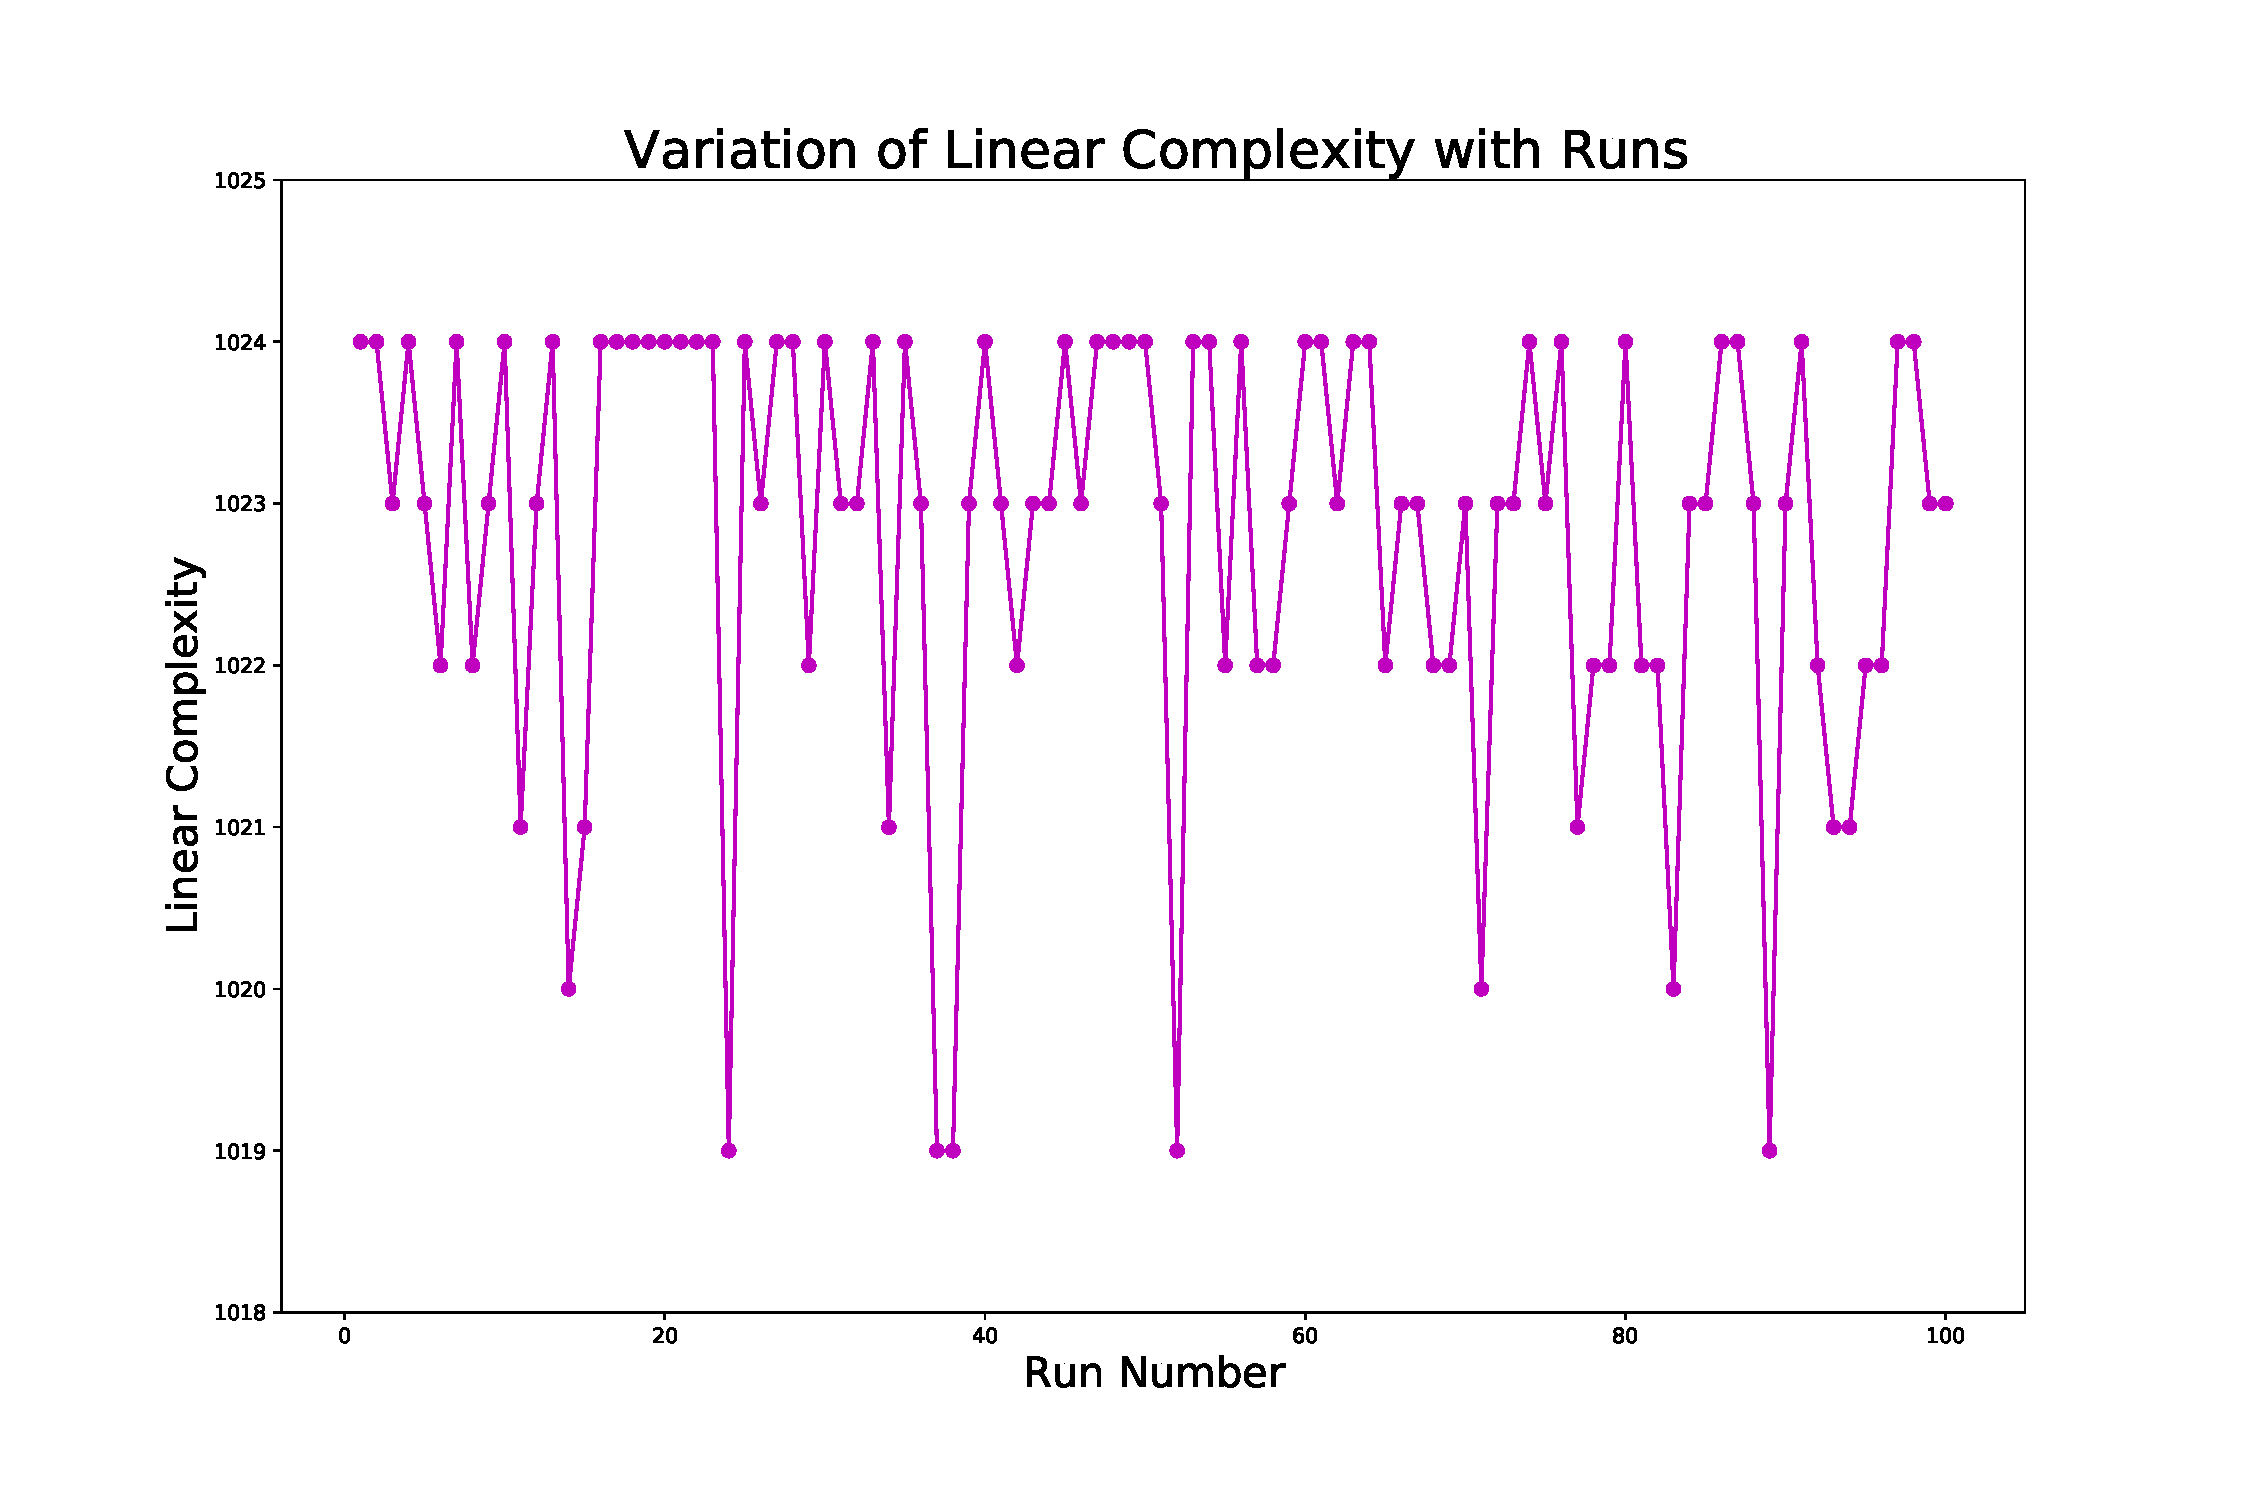
\includegraphics[width=\linewidth]{1.pdf}
        \caption{}
        \label{fig:1}
    \end{subfigure}
    \begin{subfigure}{0.48\linewidth}
        \centering
        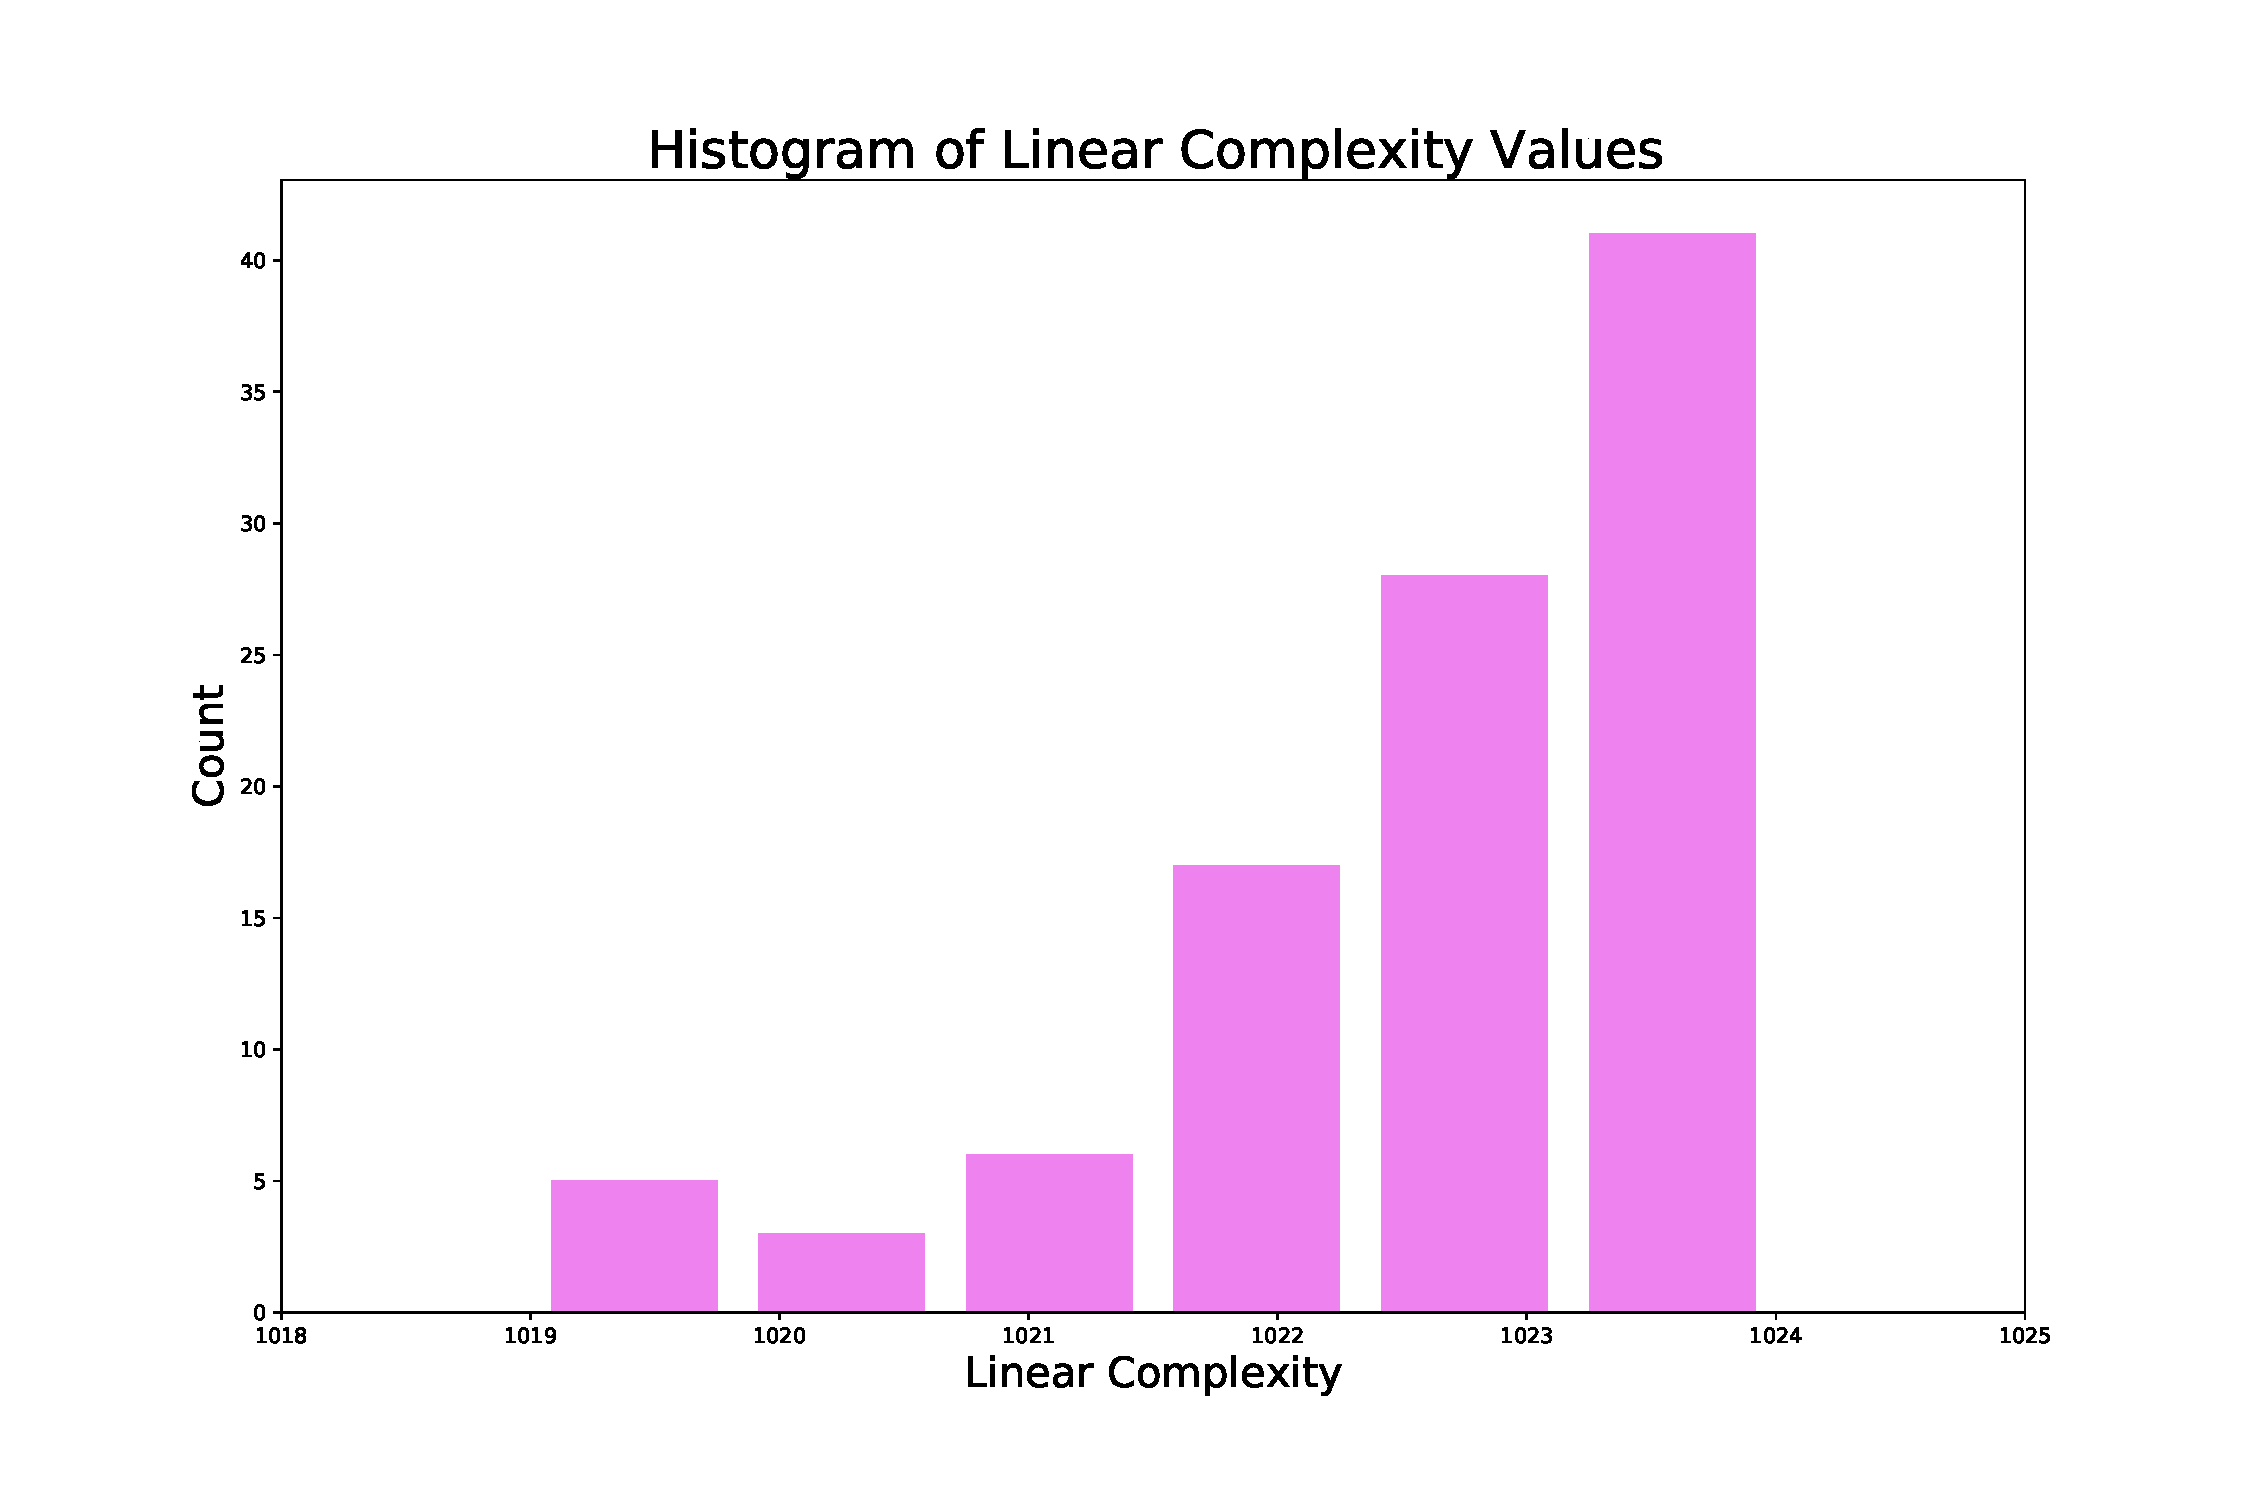
\includegraphics[width=\linewidth]{2.pdf}
        \caption{}
        \label{fig:2}
    \end{subfigure}
    \begin{subfigure}{0.48\linewidth}
        \centering
        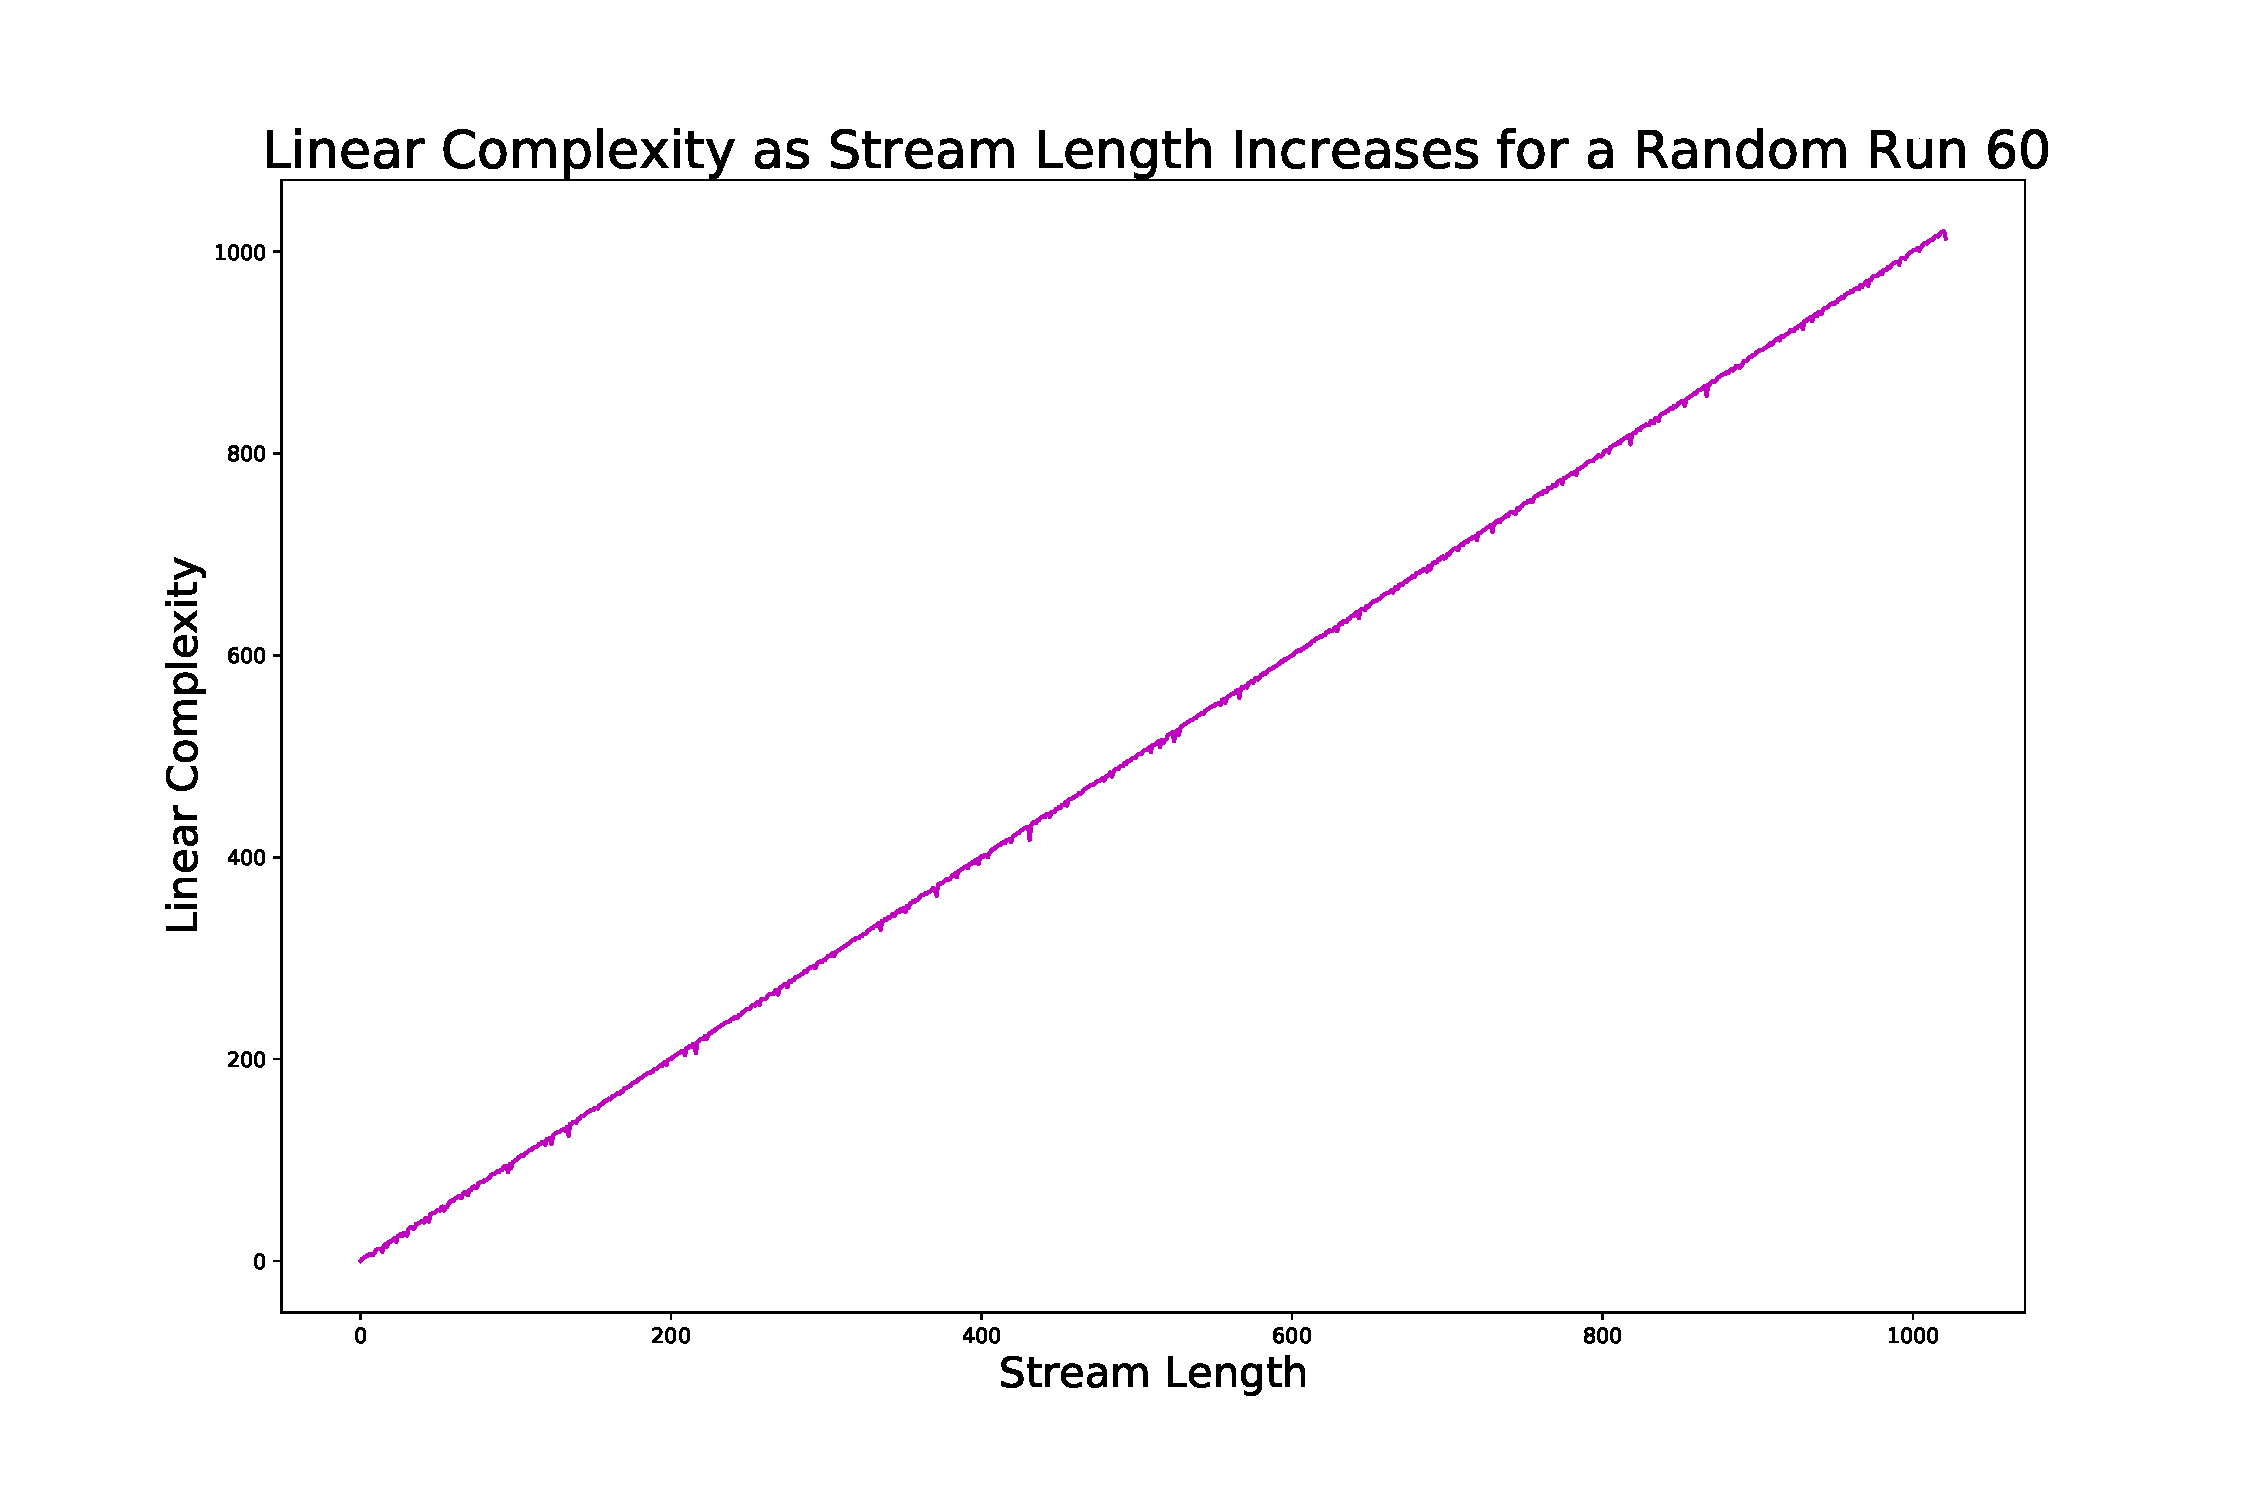
\includegraphics[width=\linewidth]{3.pdf}
        \caption{}
        \label{fig:3}
    \end{subfigure}
    \caption{Linear Complexity Plots}
    \label{fig:Q3}
\end{figure}
\begin{itemize}
    \item Figure \ref{fig:1} shows the variation of Linear Complexity (LC) for each of the 100 runs. The minimum LC is 1019 and the maximum is 1024. The LC is very high, for every run as it should be for a random keystream.
    \item Figure \ref{fig:2} is a histogram of LC values. We see that higher LC values are more frequent than lower values. This shows that our cipher is achieving the optimal LC for large number of run ($\sim 40\%$)
    \item In Figure \ref{fig:3}, a random sample from the 100 runs (run 60) was taken and the LC variation across it's length was plotted. It is clear that for every length of keystreams ($<=1024$), the achieved LC is very close to that length.
\end{itemize}
It is clear from above that the reduced size cipher generated reasonable keystreams.
\clearpage
\section{SageMath Code}
\begin{minted}[frame=single]{python}
from sage.matrix.berlekamp_massey import berlekamp_massey
import numpy as np
import bisect
import matplotlib.pyplot as plt
from matplotlib.pyplot import figure

# Function definitions
def init(key, F, register_lengths, row_count, r_1_num):
    CCSR = list(random_matrix(F, 1, register_lengths[0]+1).row(0))    # 1-indexed
    r_1 = random_matrix(F, r_1_num, register_lengths[1]+3)
    r_2 = list(random_matrix(F, 1, register_lengths[2]).row(0))
    r_3 = list(random_matrix(F, 1, register_lengths[3]).row(0))
    
    sum = np.zeros(len(row_count), dtype = int)
    sum[0] = row_count[0]
    for i in range(1, len(row_count)):
        sum[i] = row_count[i] + sum[i-1]
    
    mapping = {}
    mapping[0,0] = 0
    column_count = np.zeros(len(key)+1, dtype = int)
    column_count[0] = 1
    for i in range(1,register_lengths[0]+1):
        idx = bisect.bisect_left(sum, i)
        j = 48 + i - sum[idx]
        mapping[idx, j] = i
        column_count[j] += 1
    for i in range(2 + column_count[len(key)]):
        j = len(key) - i
        if (1, j) not in mapping:
            mapping[1, j] = 0
    
    return CCSR, r_1, r_2, r_3, mapping, column_count

def g(i, a, b, c, d):
    if i == 0:
        return a + b + c + d
    elif i == 1:
        return 1 + a + b + c * (d + 1)
    elif i == 2:
        return a * (1 + b) + c * (1 + d)
    else:
        return 0

def parameters(i,j):
    value = (j-i) % 6
    if value == 1 or value == 4:
        return 0, 2*(j-i-1)/3, j-2
    elif value == 2 or value == 5:
        return 1, j-4, j-2
    elif value == 3:
        return 1, 0, j-2
    else:
        return 1, j-5, 0

def state_update(F, key, CCSR, r_1, r_2, r_3, mapping, column_count, 
                 register_lengths, r_1_num, row_count):
    CCSR_new = list(random_matrix(F, 1, register_lengths[0]+1).row(0))    # 1-indexed
    for j in range(1, len(key)+1):
        for i in range(column_count[j]):
            x, v, w = parameters(i, j)
            if j < 3:
                v = 0
                w = 0
                c = 0
                d = 0
            a = CCSR[mapping[i%column_count[j-1], j-1]]
            b = key[j-1]
            c = CCSR[mapping[i%column_count[v], v]]
            d = CCSR[mapping[i%column_count[w], w]]
            if j == len(key):
                x = 2
                b = CCSR[mapping[0, j-1-i]]
                c = CCSR[mapping[i%column_count[j-2], j-2]]
                d = CCSR[mapping[1, j-2-i]]
            CCSR_new[mapping[i, j]] = g(x, a, b, c, d)
    CCSR = CCSR_new;
    for i in range(register_lengths[1]):
        a = CCSR[register_lengths[0] - i]
        b = CCSR[i + int(register_lengths[0] * 18/128)]
        c = CCSR[int(register_lengths[0] * 113/128) - i]
        d = CCSR[i + 1]
        r_1[0, (4*i) % register_lengths[1]] = g(1, a, b, c, d)
    for j in range(1, r_1_num):
        for i in range(register_lengths[1]):
            a = r_1[j-1, i]
            b = r_1[j-1, i+3]
            c = r_1[j-1, i+1]
            d = r_1[j-1, i+2]
            r_1[j, (4*i) % register_lengths[1]] = g(1, a, b, c, d)
    for i in range(register_lengths[2]):
        a = r_1[r_1_num-1, 4*i]
        b = r_1[r_1_num-1, 4*i+3]
        c = r_1[r_1_num-1, 4*i+1]
        d = r_1[r_1_num-1, 4*i+2]
        r_2[i] = g(1, a, b, c, d)
    for i in range(register_lengths[3]):
        a = r_2[4*i]
        b = r_2[4*i+1]
        c = r_2[4*i+2]
        d = r_2[4*i+3]
        r_3[i] = g(0, a, b, c, d)
    return CCSR, r_1, r_2, r_3

def output_stream(key, CCSR, r_1, r_2, r_3):
    return sum(r_3)

def generate_stream(F, key, IV, CCSR, r_1, r_2, r_3, mapping, column_count, 
                    register_lengths, r_1_num, row_count, size):
    key_combined = [key[i] + IV[i] for i in range(len(key))]
    output = []
    for i in range(min(size, len(key_combined))):
        output.append(key_combined[i])
    for i in range(len(key_combined), size):
        CCSR, r_1, r_2, r_3 = state_update(F, key_combined, CCSR, r_1, r_2, r_3, mapping, 
                                   column_count, register_lengths, r_1_num, row_count)
        output.append(output_stream(key, CCSR, r_1, r_2, r_3))    
    return output
def generate_data(IV_num, size):
    F = GF(2)
    register_lengths = [64, 53, 12, 3]
    r_1_num = 2
    row_count = [48, 6 , 3, 3, 1, 1, 1, 1]
    output = []
    IVs = []
    key_length = 48
    key = list(random_matrix(F, 1, key_length).row(0))
    for i in range(IV_num):
        CCSR, r_1, r_2, r_3, mapping, column_count = init(key, F, register_lengths, 
                                                  row_count, r_1_num)
        IV = list(random_matrix(F, 1, key_length).row(0))
        IVs.append(IV)
        output.append(generate_stream(F, key, IV, CCSR, r_1, r_2, r_3, mapping, 
                              column_count, register_lengths, r_1_num, row_count, size))
    return key, IVs, output

# Call functions
set_random_seed(0)
key, IVs, output = generate_data(100, 1024) # 100 is number of IVs, 1024 is stream length
linear_complexities = []
for o in output:
    linear_complexities.append(berlekamp_massey(o+o).degree())
# berlekamp_massey gives correct result when period <= half length, hence stream taken twice

# Figure 1
fig, ax = plt.subplots()
ax.plot(np.arange(1, len(linear_complexities)+1), linear_complexities, '-om')
ax.set_xlabel('Run Number', fontsize = 20)
ax.set_ylabel('Linear Complexity', fontsize = 20)
fig.set_size_inches(15, 10, forward=True)
ax.set_ylim([1018, 1025])
ax.set_title('Variation of Linear Complexity with Runs', fontsize = 25)
plt.savefig('1.pdf')

# Figure 2
bins_num = len(np.unique(linear_complexities))
fig, ax = plt.subplots()
ax.hist(linear_complexities, bins = bins_num, rwidth = 0.8, color = 'violet')
ax.set_xlabel('Linear Complexity', fontsize = 20)
ax.set_ylabel('Count', fontsize = 20)
fig.set_size_inches(15, 10, forward=True)
ax.set_xlim([1018, 1025])
ax.set_title('Histogram of Linear Complexity Values', fontsize = 25)
plt.savefig('2.pdf')

# Figure 3
r = ZZ.random_element(0,99)
linear_complexities_one = []
for i in range(2, len(output[r])):
    linear_complexities_one.append(berlekamp_massey(o[1:i]+o[1:i]).degree())
fig, ax = plt.subplots()
ax.plot(linear_complexities_one, '-m')
ax.set_xlabel('Stream Length', fontsize = 20)
ax.set_ylabel('Linear Complexity', fontsize = 20)
fig.set_size_inches(15, 10, forward=True)
ax.set_title('Linear Complexity as Stream Length Increases for a Random Run {}'.
             format(r), fontsize = 25)
plt.savefig('3.pdf')
\end{minted}
% \section{References}
% \href{https://en.wikipedia.org/wiki/Band-stop_filter}{Notch Filter - Wikipedia}\\
% \href{https://www2.humusoft.cz/www/papers/tcp09/035_hanta.pdf}{Rational Approximation of Time Delay - Hanta}
\bibliographystyle{plainurl}
\nocite{*}
\bibliography{references}
\addcontentsline{toc}{section}{References}
\end{document}